
\documentclass[a4paper,11pt]{article}
\usepackage[utf8]{inputenc}
\usepackage[T1]{fontenc}
\usepackage[english]{babel}
\usepackage[right=2.5cm, left=2.5cm, bottom=2cm, top=2cm]{geometry}
\usepackage[ddmmyyyy]{datetime}
\usepackage[table]{xcolor}
\usepackage[colorlinks=true,linkcolor=blue]{hyperref}
\usepackage{lmodern,mathptmx,changepage,titlesec,hyperref,listings,lstautogobble,graphicx,array,longtable,multirow,lipsum,tikz,shorttoc,enumitem,float}
\usetikzlibrary{arrows,automata}
\usetikzlibrary{positioning}

\renewcommand{\rmdefault}{\sfdefault} %Utilisation de la police sans-serif ("Computer Modern Sans") pour la police roman
\renewcommand{\ttdefault}{pcr} 	%Utilisation d'une police "CourrierNew" pour la police monospaced (pour faire un listing manuel)
\linespread{1.15}				%Interligne

%Utilisation de liens colorés en bleu et soulignés
\hypersetup{colorlinks=true, urlcolor=blue, urlbordercolor=blue, linkcolor=black, linkbordercolor=white}
\makeatletter \Hy@AtBeginDocument{\def\@pdfborder{0 0 1} \def\@pdfborderstyle{/S/U/W 1}}\makeatother

\titlespacing*{\section} {0cm}{7ex plus 1ex minus .2ex}{1.5ex plus .2ex}
\titlespacing*{\subsection} {0cm}{4.5ex plus 1ex minus .2ex}{1.5ex plus .2ex}
\titleformat*{\section}{\LARGE\bfseries}
\titleformat*{\subsection}{\large\bfseries}
\titleformat*{\subsubsection}{\normalsize\bfseries}

\definecolor{darkgreen}{rgb}{0,0.8,0}
\definecolor{mygray}{rgb}{0.93,0.93,0.93}
\definecolor{mymauve}{rgb}{0.58,0,0.82}
\lstset{	
	language=fortran,
	basicstyle=\small\ttfamily,
	backgroundcolor=\color{white},
	breaklines=true,
	breakatwhitespace=true,
	tabsize=3,
	frame=none,
	rulecolor=\color{black},
	keywordstyle=\color{blue}\bfseries,
	stringstyle=\color{orange},
	showstringspaces=false,
	commentstyle=\footnotesize\color{darkgreen},
	keepspaces=true,
	extendedchars=true,
	numbers=none,
	numberstyle=\tiny\color{lightgray},
	stepnumber=1,
	escapeinside={(@}{@)},
	autogobble=true,
	literate=
		{á}{{\'a}}1 {é}{{\'e}}1 {í}{{}}1 {ó}{{\'o}}1 {ú}{{\'u}}1
		{Á}{{\'A}}1 {É}{{\'E}}1 {Í}{{\'I}}1 {Ó}{{\'O}}1 {Ú}{{\'U}}1
		{à}{{\`a}}1 {è}{{\`e}}1 {ì}{{\`i}}1 {ò}{{\`o}}1 {ù}{{\`u}}1
		{À}{{\`A}}1 {È}{{\'E}}1 {Ì}{{\`I}}1 {Ò}{{\`O}}1 {Ù}{{\`U}}1
		{ä}{{\"a}}1 {ë}{{\"e}}1 {ï}{{\"i}}1 {ö}{{\"o}}1 {ü}{{\"u}}1
		{Ä}{{\"A}}1 {Ë}{{\"E}}1 {Ï}{{\"I}}1 {Ö}{{\"O}}1 {Ü}{{\"U}}1
		{â}{{\^a}}1 {ê}{{\^e}}1 {î}{{\^i}}1 {ô}{{\^o}}1 {û}{{\^u}}1
		{Â}{{\^A}}1 {Ê}{{\^E}}1 {Î}{{\^I}}1 {Ô}{{\^O}}1 {Û}{{\^U}}1
		{œ}{{\oe}}1 {Œ}{{\OE}}1 {æ}{{\ae}}1 {Æ}{{\AE}}1 {ß}{{\ss}}1
		{ç}{{\c c}}1 {Ç}{{\c C}}1 {ø}{{\o}}1 {å}{{\r a}}1 {Å}{{\r A}}1
		{€}{{e}}1 {£}{{\pounds}}1 {«}{{\guillemotleft}}1
		{»}{{\guillemotright}}1 {ñ}{{\~n}}1 {Ñ}{{\~N}}1 {¿}{{?`}}1
}

%Redéfinition de la taille de \Huge pour le titre du document
\makeatletter\renewcommand\Huge{\@setfontsize\Huge{37pt}{40}}\makeatother
\date{\today}

\usepackage{listings}
\usepackage{algorithm}
\usepackage{amsmath} 
\usepackage{algorithmic}
\usepackage{array,multirow,makecell}
\usepackage[table]{xcolor}

\usepackage[T1]{fontenc}
\usepackage[utf8]{inputenc}
\usepackage{multicol}


\usepackage{fancyhdr}
\pagestyle{fancy}
%\setlength{\unitlength}{1mm}
%\addtolength{\headheight}{1.5\baselineskip}
\renewcommand{\headrulewidth}{0pt}
\renewcommand{\footrulewidth}{0pt}
\rhead{

\includegraphics[width=4.5cm]{tex/scale.png}
}


%\author{Agenium Scale}
\title{
\includegraphics[width=27em]{tex/scale.png}\\ \vspace{9em}{\fontsize{30}{40} \textbf{Benchmarks of NSIMD on Intel Skylake/AVX-512 capable chip}}}
\begin{document}
\maketitle
\vspace{10em}
\textbf{AGENIUM SCALE}\\
Rue Noetzlin\\
Batiment 660, Digiteo Labs\\
91 190 Gif-sur-Yvette\\
01 69 15 32 32 \\
contact@numsclae.com\\
https://www.numscale.com\\

\clearpage
\pagenumbering{gobble}

\begin{flushright}\textit{}\end{flushright}


\tableofcontents
\newpage
\section{Introduction} %(SOME PAGES)
	\subsection{About this document}
 This document presents the results of benchmarks performed by AGNENIUM SCALE on Intel Skylake/AVX-512 capable chip.\\
 
	This document is meant to be read by software developers.  The explanations provided in thepresent  sections  are  not  intended  to  be  detailed.   We  assume  that  the  reader  has  sufficientknowledge to understand the present document.  If you have any relevant question feel free to contact us at \href{contact@numscale.com}{contact@numscale.com}. \\
 
 This first part of this document is the introduction which provides detailed information about the benchmarking setup, such as hardware, software, and metrics used.  The second part gives benchmark results that allow you to have a quick idea of how NSIMD performs against other GROMACS versions. The third part provides the comparaison of the performances between NSIMD and the others SIMD extension.\\
 
 For the benchmarks performed, the version of gromacs is 2019.3 published on june 2019. However, the version used has several modifications to integrate NSIMD into the source code. You will find it at  \href{https://github.com/agenium-scale/gromacs}{https://github.com/agenium-scale/gromacs}. You can see the corrections and the differents additions to the NSIMD version on the nsimd-translate branch in this fork of the GROMACS's repository.
 
	\subsection{Benchmark Setup}
	
	All benchmarks are performed using tools given by GROMACS for testings the performace. For each benchmarks we have use \textit{gmx tune\_pme} with only one MPI rank. For more information on \textit{gmx tune\_pme} please see: \\\href{http://manual.gromacs.org/documentation/2018/onlinehelp/gmx-tune\_pme.html}{http://manual.gromacs.org/documentation/2018/onlinehelp/gmx-tune\_pme.html}.\\
	
	For the benchmark runs, the default of 1000 time steps should suffice for most systems. The dynamic load balancing needs about 100 time steps to adapt to local load imbalances, therefore the time step counters are by default reset after 100 steps. \\
	
	After calling \textit{gmx\_mpi mdrun} several times (option \textit{-r} repeat each test \textit{r} times), detailed performance information is available in the output file \textit{perf.out}. Note that during the benchmarks, a couple of temporary files are created and are deleted after each test. 
	
	\subsection{Contents of this document}
	
	In the following section we dump the outputs of some well-known shell commands that pro-vide useful information on the machine, operating system, compiler version, that were used forbenchmarks. Dumps of shell commands have two main advantages:
	
	\begin{itemize}
	\item Very accurate information about the benchmarking environment is provided in raw formideal for our intended audience.
	\item We do not have time to write some cumbersome code to generate beautiful English sentencesto describe what is best described by shell commands whose output format is well knownby our intended audience.
	\end{itemize}
	
		
	\subsection{Organization of benchmarks} 
	
For each SIMD extensions used, the following benchmarks are performed:
	
	\begin{itemize}
	\item The report made by GROMACS are given below for each SIMD extension tested (SSE2, SSE4.1, AVX, AVX2 and AVX 512 Skylake) and NSIMD. 
	
	\item This report provides information on the number of MPI rank used, on the input file and the command used to launch the benchmark. There is also information on the simulation time in nanosecond per day (Higher is better) as well as the number of cycles for each PME rank. In addition, it is indicated which PME rank is the most recommended for better performance during the simulation.

	\item The essentials results information are extracted from this previous report (The average for the simulation time and the number of cycles). 
	
	\item A performance comparison between NSIMD and every SIMD extensions used during the benchmarks.
	\end{itemize}
	
	\subsection{Compiler version}
	\begin{lstlisting}[frame=single]
gcc (Debian 8.3.0-6) 8.3.0
Copyright (C) 2018 Free Software Foundation, Inc.
This is free software; see the source for copying conditions.  There is NO
warranty; not even for MERCHANTABILITY or FITNESS FOR A PARTICULAR PURPOSE.
\end{lstlisting}
	
	\subsection{Operating system description}
\begin{lstlisting}[frame=single]
Linux glastonbury 4.19.0-1-amd64 #1 SMP Debian 4.19.12-1 (2018-12-22) x86_64 GNU/Linux
\end{lstlisting}
	\subsection{Information about the CPU architecture}
	\begin{lstlisting}[frame=single]
Architecture:        x86_64
CPU op-mode(s):      32-bit, 64-bit
Byte Order:          Little Endian
Address sizes:       46 bits physical, 48 bits virtual
CPU(s):              32
On-line CPU(s) list: 0-31
Thread(s) per core:  2
Core(s) per socket:  8
Socket(s):           2
NUMA node(s):        2
Vendor ID:           GenuineIntel
CPU family:          6
Model:               85
Model name:          Intel(R) Xeon(R) Silver 4110 CPU @ 2.10GHz
Stepping:            4
CPU MHz:             800.681
BogoMIPS:            4200.00
Virtualization:      VT-x
L1d cache:           32K
L1i cache:           32K
L2 cache:            1024K
L3 cache:            11264K
NUMA node0 CPU(s):   0-7,16-23
NUMA node1 CPU(s):   8-15,24-31
Flags:               fpu vme de pse tsc msr pae mce cx8 apic sep mtrr pge mca cmov pat pse36 clflush dts acpi mmx fxsr sse sse2 ss ht tm pbe syscall nx pdpe1gb rdtscp lm constant_tsc art arch_perfmon pebs bts rep_good nopl xtopology nonstop_tsc cpuid aperfmperf pni pclmulqdq dtes64 ds_cpl vmx smx est tm2 ssse3 sdbg fma cx16 xtpr pdcm pcid dca sse4_1 sse4_2 x2apic movbe popcnt tsc_deadline_timer aes xsave avx f16c rdrand lahf_lm abm 3dnowprefetch cpuid_fault epb cat_l3 cdp_l3 invpcid_single pti intel_ppin mba tpr_shadow vnmi flexpriority ept vpid ept_ad fsgsbase tsc_adjust bmi1 hle avx2 smep bmi2 erms invpcid rtm cqm mpx rdt_a avx512f avx512dq rdseed adx smap clflushopt clwb intel_pt avx512cd avx512bw avx512vl xsaveopt xsavec xgetbv1 xsaves cqm_llc cqm_occup_llc cqm_mbm_total cqm_mbm_local dtherm ida arat pln pts hwp_epp pku ospke
\end{lstlisting}
	
	\subsection{Information about the RAM}
	\begin{lstlisting}[frame=single]
MemTotal:       181106648 kB
MemFree:        116730512 kB
MemAvailable:   176785980 kB
Buffers:         2837728 kB
Cached:         55357572 kB
SwapCached:            0 kB
Active:         12591656 kB
Inactive:       45843992 kB
Active(anon):     381476 kB
Inactive(anon):  1623940 kB
Active(file):   12210180 kB
Inactive(file): 44220052 kB
Unevictable:           0 kB
Mlocked:               0 kB
SwapTotal:             0 kB
SwapFree:              0 kB
Dirty:                28 kB
Writeback:             0 kB
AnonPages:        238436 kB
Mapped:           234284 kB
Shmem:           1765072 kB
Slab:            5388084 kB
SReclaimable:    4988952 kB
SUnreclaim:       399132 kB
KernelStack:        7120 kB
PageTables:         3412 kB
NFS_Unstable:          0 kB
Bounce:                0 kB
WritebackTmp:          0 kB
CommitLimit:    90553324 kB
Committed_AS:    2151012 kB
VmallocTotal:   34359738367 kB
VmallocUsed:           0 kB
VmallocChunk:          0 kB
Percpu:           109184 kB
HardwareCorrupted:     0 kB
AnonHugePages:    178176 kB
ShmemHugePages:        0 kB
ShmemPmdMapped:        0 kB
HugePages_Total:       0
HugePages_Free:        0
HugePages_Rsvd:        0
HugePages_Surp:        0
Hugepagesize:       2048 kB
Hugetlb:               0 kB
DirectMap4k:     1675868 kB
DirectMap2M:    52379648 kB
DirectMap1G:    132120576 kB
	\end{lstlisting}

\subsection{Information about the standard library}
%ldd --version	
\begin{lstlisting}[frame=single] 
ldd (Debian GLIBC 2.28-10) 2.28
Copyright (C) 2018 Free Software Foundation, Inc.
This is free software; see the source for copying conditions.  There is NO
warranty; not even for MERCHANTABILITY or FITNESS FOR A PARTICULAR PURPOSE.
Written by Roland McGrath and Ulrich Drepper.
\end{lstlisting}
	
\section{Benchmarks results} %(5x2)

In the first time we will give the report given by GROMACS on the performance tests for each SIMD extension and NSIMD. Then the relevant information obtained will be extracted at a second time. And finally we will give the comparison between the basic version of GROMACS and with the NSIMD version. The presented results will demonstrate  that the versions of NSIMD have almost the same performance as the native versions.
 
\subsection{Performance tests beetween SSE2 and NSIMD for SSE2}
\subsubsection{SSE2}
GROMACS report: \\
\begin{lstlisting}[frame=single]

------------------------------------------------------------

      P E R F O R M A N C E   R E S U L T S

------------------------------------------------------------
gmx tune_pme for GROMACS 2020-dev-20190716-2e535c390-dirty-unknown
Number of ranks         : 1
The mpirun command is   : mpirun
Passing # of ranks via  : -np
The mdrun  command is   : ../build/bin/gmx_mpi mdrun
mdrun args benchmarks   : -resetstep 1500 -o bench.trr -x bench.xtc -cpo bench.cpt -c bench.gro -e bench.edr -g bench.log 
Benchmark steps         : 1000
dlb equilibration steps : 1500
mdrun args at launchtime: 
Repeats for each test   : 10
Input file              : topol.tpr
   PME/PP load estimate : 0.999978
   Number of particles  : 6
   Coulomb type         : PME
   Grid spacing x y z   : 0.115742 0.115742 0.115742
   Van der Waals type   : Cut-off

Will try these real/reciprocal workload settings:
 No.   scaling  rcoulomb  nkx  nky  nkz   spacing      rvdw  tpr file
   0  1.000000  1.000000  108  108  108  0.120000   1.000000  topol_bench00.tpr

Individual timings for input file 0 (topol_bench00.tpr):
PME ranks      Gcycles       ns/day        PME/f    Remark
   0          2350.243        2.467          -      OK.
   0          2427.413        2.389          -      OK.
   0          2412.697        2.403          -      OK.
   0          2442.498        2.374          -      OK.
   0          2341.577        2.476          -      OK.
   0          2298.972        2.522          -      OK.
   0          2288.342        2.534          -      OK.
   0          2307.032        2.513          -      OK.
   0          2291.177        2.531          -      OK.
   0          2296.336        2.525          -      OK.
  -1( -1)     2301.922        2.519          -      OK.
  -1( -1)     2303.064        2.518          -      OK.
  -1( -1)     2290.594        2.531          -      OK.
  -1( -1)     2295.430        2.526          -      OK.
  -1( -1)     2298.698        2.522          -      OK.
  -1( -1)     2322.819        2.496          -      OK.
  -1( -1)     2325.540        2.493          -      OK.
  -1( -1)     2325.342        2.493          -      OK.
  -1( -1)     2320.427        2.499          -      OK.
  -1( -1)     2317.554        2.502          -      OK.

Tuning took    30.0 minutes.

------------------------------------------------------------
Summary of successful runs:
Line tpr PME ranks  Gcycles Av.     Std.dev.       ns/day        PME/f
   0   0    0          2345.629       60.508        2.473          -  
   1   0   -1( -1)     2310.139       13.486        2.510          -  

------------------------------------------------------------
Best performance was achieved with the automatic number of PME ranks (see line 1)
Please use this command line to launch the simulation:

mpirun -np 1 ../build/bin/gmx_mpi mdrun -npme -1 -s topol.tpr  
------------------------------------------------------------

\end{lstlisting}

Relevant information:
\begin{center}
    \begin{tabular}{|p{3.5cm}|p{3.5cm}|p{3.5cm}|p{3.5cm}|} \hline
         PME ranks & Gcycles Average & Std.dev. & ns/day \\ \hline
         0 & 2345.629  & 60.508  & 2.473  \\ \hline
         -1 (-1) & 2310.139 & 13.486 & 2.510  \\ \hline
    \end{tabular}
    \begin{tabular}{|p{3.5cm}|p{11.4cm}|} \hline
         Run Time (min) & 30.0 \\ \hline
    \end{tabular}
\end{center}

\subsubsection{NSIMD for SSE2}
GROMACS report: \\
\begin{lstlisting}[frame=single]

------------------------------------------------------------

      P E R F O R M A N C E   R E S U L T S

------------------------------------------------------------
gmx tune_pme for GROMACS 2020-dev-20190716-2e535c390-dirty-unknown
Number of ranks         : 1
The mpirun command is   : mpirun
Passing # of ranks via  : -np
The mdrun  command is   : ../build/bin/gmx_mpi mdrun
mdrun args benchmarks   : -resetstep 1500 -o bench.trr -x bench.xtc -cpo bench.cpt -c bench.gro -e bench.edr -g bench.log 
Benchmark steps         : 1000
dlb equilibration steps : 1500
mdrun args at launchtime: 
Repeats for each test   : 10
Input file              : topol.tpr
   PME/PP load estimate : 0.999978
   Number of particles  : 6
   Coulomb type         : PME
   Grid spacing x y z   : 0.115742 0.115742 0.115742
   Van der Waals type   : Cut-off

Will try these real/reciprocal workload settings:
 No.   scaling  rcoulomb  nkx  nky  nkz   spacing      rvdw  tpr file
   0  1.000000  1.000000  108  108  108  0.120000   1.000000  topol_bench00.tpr

Individual timings for input file 0 (topol_bench00.tpr):
PME ranks      Gcycles       ns/day        PME/f    Remark
   0          2327.227        2.491          -      OK.
   0          2292.502        2.529          -      OK.
   0          2294.212        2.527          -      OK.
   0          2290.497        2.531          -      OK.
   0          2310.354        2.510          -      OK.
   0          2297.936        2.523          -      OK.
   0          2296.340        2.525          -      OK.
   0          2308.574        2.512          -      OK.
   0          2297.881        2.523          -      OK.
   0          2300.145        2.521          -      OK.
  -1( -1)     2310.168        2.510          -      OK.
  -1( -1)     2311.627        2.508          -      OK.
  -1( -1)     2291.752        2.530          -      OK.
  -1( -1)     2309.331        2.511          -      OK.
  -1( -1)     2300.161        2.521          -      OK.
  -1( -1)     2302.002        2.519          -      OK.
  -1( -1)     2306.201        2.514          -      OK.
  -1( -1)     2294.641        2.527          -      OK.
  -1( -1)     2292.854        2.529          -      OK.
  -1( -1)     2304.064        2.516          -      OK.

Tuning took    29.6 minutes.

------------------------------------------------------------
Summary of successful runs:
Line tpr PME ranks  Gcycles Av.     Std.dev.       ns/day        PME/f
   0   0    0          2301.567       11.054        2.519          -  
   1   0   -1( -1)     2302.280        7.307        2.518          -  

------------------------------------------------------------
Best performance was achieved with 0 PME ranks (see line 0)
Please use this command line to launch the simulation:

mpirun -np 1 ../build/bin/gmx_mpi mdrun -npme 0 -s topol.tpr  
------------------------------------------------------------

\end{lstlisting}

Relevant information:
\begin{center}
    \begin{tabular}{|p{3.5cm}|p{3.5cm}|p{3.5cm}|p{3.5cm}|} \hline
         PME ranks & Gcycles Average & Std.dev. & ns/day \\ \hline
         0 & 2301.567  & 11.054  & 2.519  \\ \hline
         -1 (-1) & 2302.280 & 7.307 & 2.518  \\ \hline
    \end{tabular}
    \begin{tabular}{|p{3.5cm}|p{11.4cm}|} \hline
         Run Time (min) & 30.0 \\ \hline
    \end{tabular}
\end{center}
\subsubsection{Comparison of results}

\begin{figure}[!h]
\centering
        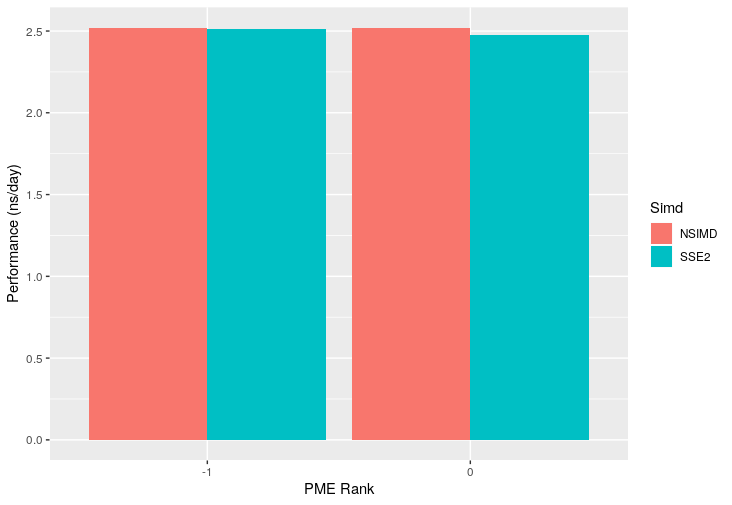
\includegraphics[scale=0.8]{SSE2.png}
        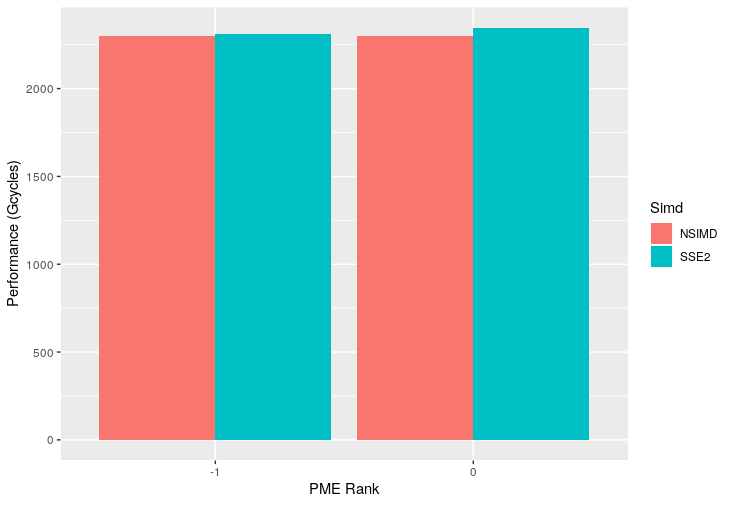
\includegraphics[scale=0.8]{SSE2_2.png}
        \caption{GROMACS Performance between SSE2 and NSIMD}
        \label{fg:f1}
\end{figure}
\newpage

\subsection{Performance tests between SSE4.1 and NSIMD}
\subsubsection{SSE4.1}
\begin{lstlisting}[frame=single]

------------------------------------------------------------

      P E R F O R M A N C E   R E S U L T S

------------------------------------------------------------
gmx tune_pme for GROMACS 2020-dev-20190716-2e535c390-dirty-unknown
Number of ranks         : 1
The mpirun command is   : mpirun
Passing # of ranks via  : -np
The mdrun  command is   : ../build/bin/gmx_mpi mdrun
mdrun args benchmarks   : -resetstep 1500 -o bench.trr -x bench.xtc -cpo bench.cpt -c bench.gro -e bench.edr -g bench.log 
Benchmark steps         : 1000
dlb equilibration steps : 1500
mdrun args at launchtime: 
Repeats for each test   : 10
Input file              : topol.tpr
   PME/PP load estimate : 0.999978
   Number of particles  : 6
   Coulomb type         : PME
   Grid spacing x y z   : 0.115742 0.115742 0.115742
   Van der Waals type   : Cut-off

Will try these real/reciprocal workload settings:
 No.   scaling  rcoulomb  nkx  nky  nkz   spacing      rvdw  tpr file
   0  1.000000  1.000000  108  108  108  0.120000   1.000000  topol_bench00.tpr

Individual timings for input file 0 (topol_bench00.tpr):
PME ranks      Gcycles       ns/day        PME/f    Remark
   0          2316.736        2.503          -      OK.
   0          2312.407        2.507          -      OK.
   0          2318.358        2.501          -      OK.
   0          2302.580        2.518          -      OK.
   0          2296.213        2.525          -      OK.
   0          2292.474        2.529          -      OK.
   0          2294.912        2.527          -      OK.
   0          2304.831        2.516          -      OK.
   0          2292.868        2.529          -      OK.
   0          2324.951        2.494          -      OK.
  -1( -1)     2317.890        2.501          -      OK.
  -1( -1)     2323.069        2.496          -      OK.
  -1( -1)     2313.187        2.507          -      OK.
  -1( -1)     2302.052        2.519          -      OK.
  -1( -1)     2294.498        2.527          -      OK.
  -1( -1)     2289.775        2.532          -      OK.
  -1( -1)     2309.190        2.511          -      OK.
  -1( -1)     2291.554        2.530          -      OK.
  -1( -1)     2290.885        2.531          -      OK.
  -1( -1)     2295.862        2.525          -      OK.

Tuning took    29.7 minutes.

------------------------------------------------------------
Summary of successful runs:
Line tpr PME ranks  Gcycles Av.     Std.dev.       ns/day        PME/f
   0   0    0          2305.633       11.804        2.515          -  
   1   0   -1( -1)     2302.796       12.216        2.518          -  

------------------------------------------------------------
Best performance was achieved with the automatic number of PME ranks (see line 1)
Please use this command line to launch the simulation:

mpirun -np 1 ../build/bin/gmx_mpi mdrun -npme -1 -s topol.tpr  
------------------------------------------------------------

\end{lstlisting}

Relevant information:
\begin{center}
    \begin{tabular}{|p{3.5cm}|p{3.5cm}|p{3.5cm}|p{3.5cm}|} \hline
         PME ranks & Gcycles Average & Std.dev. & ns/day \\ \hline
         0 & 2305.633  & 11.804  & 2.515  \\ \hline
         -1 (-1) & 2302.796 & 12.216 & 2.518  \\ \hline
    \end{tabular}
    \begin{tabular}{|p{3.5cm}|p{11.4cm}|} \hline
         Run Time (min) & 29.7 \\ \hline
    \end{tabular}
\end{center}

\subsubsection{NSIMD for SSE4.1}
\begin{lstlisting}[frame=single]
------------------------------------------------------------

      P E R F O R M A N C E   R E S U L T S

------------------------------------------------------------
gmx tune_pme for GROMACS 2020-dev-20190716-2e535c390-dirty-unknown
Number of ranks         : 1
The mpirun command is   : mpirun
Passing # of ranks via  : -np
The mdrun  command is   : ./bin/gmx_mpi mdrun
mdrun args benchmarks   : -resetstep 1500 -o bench.trr -x bench.xtc -cpo bench.cpt -c bench.gro -e bench.edr -g bench.log 
Benchmark steps         : 1000
dlb equilibration steps : 1500
mdrun args at launchtime: 
Repeats for each test   : 10
Input file              : ../benches/topol.tpr
   PME/PP load estimate : 0.999978
   Number of particles  : 6
   Coulomb type         : PME
   Grid spacing x y z   : 0.115742 0.115742 0.115742
   Van der Waals type   : Cut-off

Will try these real/reciprocal workload settings:
 No.   scaling  rcoulomb  nkx  nky  nkz   spacing      rvdw  tpr file
   0  1.000000  1.000000  108  108  108  0.120000   1.000000  ../benches/topol_bench00.tpr

Individual timings for input file 0 (../benches/topol_bench00.tpr):
PME ranks      Gcycles       ns/day        PME/f    Remark
   0          2317.930        2.501          -      OK.
   0          2300.510        2.520          -      OK.
   0          2298.326        2.523          -      OK.
   0          2301.094        2.520          -      OK.
   0          2299.800        2.521          -      OK.
   0          2330.784        2.488          -      OK.
   0          2329.806        2.489          -      OK.
   0          2338.370        2.480          -      OK.
   0          2335.475        2.483          -      OK.
   0          2304.390        2.516          -      OK.
  -1( -1)     2302.641        2.518          -      OK.
  -1( -1)     2305.711        2.515          -      OK.
  -1( -1)     2301.583        2.519          -      OK.
  -1( -1)     2298.349        2.523          -      OK.
  -1( -1)     2309.179        2.511          -      OK.
  -1( -1)     2300.231        2.521          -      OK.
  -1( -1)     2323.899        2.495          -      OK.
  -1( -1)     2323.653        2.495          -      OK.
  -1( -1)     2318.340        2.501          -      OK.
  -1( -1)     2322.351        2.497          -      OK.

Tuning took    30.2 minutes.

------------------------------------------------------------
Summary of successful runs:
Line tpr PME ranks  Gcycles Av.     Std.dev.       ns/day        PME/f
   0   0    0          2315.648       16.543        2.504          -  
   1   0   -1( -1)     2310.594       10.400        2.510          -  

------------------------------------------------------------

\end{lstlisting}

Relevant information:
\begin{center}
    \begin{tabular}{|p{3.5cm}|p{3.5cm}|p{3.5cm}|p{3.5cm}|} \hline
         PME ranks & Gcycles Average & Std.dev. & ns/day \\ \hline
         0 & 2315.648  & 16.543  & 2.504  \\ \hline
         -1 (-1) & 2310.594 & 10.400 & 2.510  \\ \hline
    \end{tabular}
    \begin{tabular}{|p{3.5cm}|p{11.4cm}|} \hline
         Run Time (min) & 30.2 \\ \hline
    \end{tabular}
\end{center}
\subsubsection{Comparison of results}

\begin{figure}[!h]
\centering
        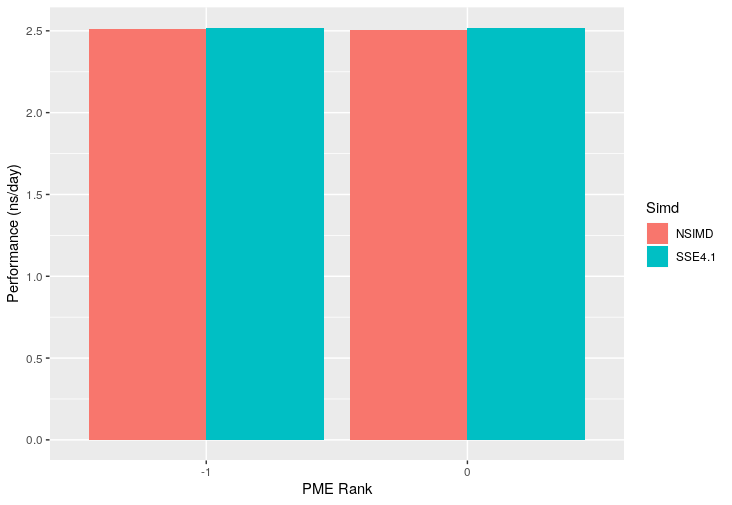
\includegraphics[scale=0.8]{SSE41.png}
        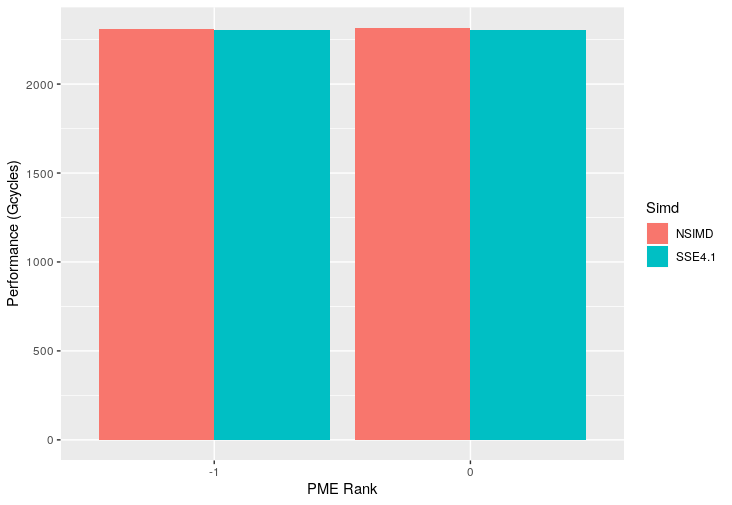
\includegraphics[scale=0.8]{SSE41_2.png}
        \caption{GROMACS Performance between SSE4.1 and NSIMD}
        \label{fg:f2}
\end{figure}
\newpage


\subsection{Performance tests beetween AVX and NSIMD for AVX}
\subsubsection{AVX}
GROMACS report: \\
\begin{lstlisting}[frame=single]

------------------------------------------------------------

      P E R F O R M A N C E   R E S U L T S

------------------------------------------------------------
gmx tune_pme for GROMACS 2020-dev-20190716-2e535c390-dirty-unknown
Number of ranks         : 1
The mpirun command is   : mpirun
Passing # of ranks via  : -np
The mdrun  command is   : ./bin/gmx_mpi mdrun
mdrun args benchmarks   : -resetstep 1500 -o bench.trr -x bench.xtc -cpo bench.cpt -c bench.gro -e bench.edr -g bench.log 
Benchmark steps         : 1000
dlb equilibration steps : 1500
mdrun args at launchtime: 
Repeats for each test   : 10
Input file              : ../benches/topol.tpr
   PME/PP load estimate : 0.999977
   Number of particles  : 6
   Coulomb type         : PME
   Grid spacing x y z   : 0.115742 0.115742 0.115742
   Van der Waals type   : Cut-off

Will try these real/reciprocal workload settings:
 No.   scaling  rcoulomb  nkx  nky  nkz   spacing      rvdw  tpr file
   0  1.000000  1.000000  108  108  108  0.120000   1.000000  ../benches/topol_bench00.tpr

Individual timings for input file 0 (../benches/topol_bench00.tpr):
PME ranks      Gcycles       ns/day        PME/f    Remark
   0          2371.440        2.445          -      OK.
   0          2347.202        2.470          -      OK.
   0          2347.959        2.469          -      OK.
   0          2334.820        2.483          -      OK.
   0          2341.169        2.477          -      OK.
   0          2334.178        2.484          -      OK.
   0          2338.660        2.479          -      OK.
   0          2344.736        2.473          -      OK.
   0          2346.047        2.471          -      OK.
   0          2344.896        2.473          -      OK.
  -1( -1)     2328.171        2.490          -      OK.
  -1( -1)     2340.642        2.477          -      OK.
  -1( -1)     2335.325        2.483          -      OK.
  -1( -1)     2333.859        2.484          -      OK.
  -1( -1)     2339.243        2.479          -      OK.
  -1( -1)     2335.493        2.483          -      OK.
  -1( -1)     2336.434        2.482          -      OK.
  -1( -1)     2346.790        2.471          -      OK.
  -1( -1)     2354.957        2.462          -      OK.
  -1( -1)     2375.184        2.441          -      OK.

Tuning took    30.2 minutes.

------------------------------------------------------------
Summary of successful runs:
Line tpr PME ranks  Gcycles Av.     Std.dev.       ns/day        PME/f
   0   0    0          2345.111       10.485        2.472          -  
   1   0   -1( -1)     2342.610       13.635        2.475          -  

------------------------------------------------------------
Best performance was achieved with the automatic number of PME ranks (see line 1)
Please use this command line to launch the simulation:

mpirun -np 1 ./bin/gmx_mpi mdrun -npme -1 -s ../benches/topol.tpr  
------------------------------------------------------------

\end{lstlisting}

Relevant information:
\begin{center}
    \begin{tabular}{|p{3.5cm}|p{3.5cm}|p{3.5cm}|p{3.5cm}|} \hline
         PME ranks & Gcycles Average & Std.dev. & ns/day \\ \hline
         0 & 2345.111  & 10.485  & 2.472  \\ \hline
         -1 (-1) & 2342.610 & 13.635 & 2.475  \\ \hline
    \end{tabular}
    \begin{tabular}{|p{3.5cm}|p{11.4cm}|} \hline
         Run Time (min) & 30.2 \\ \hline
    \end{tabular}
\end{center}

\subsubsection{NSIMD for AVX}
GROMACS report: \\
\begin{lstlisting}[frame=single]

------------------------------------------------------------

      P E R F O R M A N C E   R E S U L T S

------------------------------------------------------------
gmx tune_pme for GROMACS 2020-dev-20190716-2e535c390-dirty-unknown
Number of ranks         : 1
The mpirun command is   : mpirun
Passing # of ranks via  : -np
The mdrun  command is   : ../build/bin/gmx_mpi mdrun
mdrun args benchmarks   : -resetstep 1500 -o bench.trr -x bench.xtc -cpo bench.cpt -c bench.gro -e bench.edr -g bench.log 
Benchmark steps         : 1000
dlb equilibration steps : 1500
mdrun args at launchtime: 
Repeats for each test   : 5
Input file              : topol.tpr
   PME/PP load estimate : 0.999977
   Number of particles  : 6
   Coulomb type         : PME
   Grid spacing x y z   : 0.115742 0.115742 0.115742
   Van der Waals type   : Cut-off

Will try these real/reciprocal workload settings:
 No.   scaling  rcoulomb  nkx  nky  nkz   spacing      rvdw  tpr file
   0  1.000000  1.000000  108  108  108  0.120000   1.000000  topol_bench00.tpr

Individual timings for input file 0 (topol_bench00.tpr):
PME ranks      Gcycles       ns/day        PME/f    Remark
   0          2333.639        2.485          -      OK.
   0          2339.271        2.479          -      OK.
   0          2331.268        2.487          -      OK.
   0          2309.782        2.510          -      OK.
   0          2303.773        2.517          -      OK.
  -1( -1)     2300.292        2.521          -      OK.
  -1( -1)     2310.477        2.510          -      OK.
  -1( -1)     2299.312        2.522          -      OK.
  -1( -1)     2297.772        2.523          -      OK.
  -1( -1)     2315.438        2.504          -      OK.

Tuning took    14.9 minutes.

------------------------------------------------------------
Summary of successful runs:
Line tpr PME ranks  Gcycles Av.     Std.dev.       ns/day        PME/f
   0   0    0          2323.547       15.726        2.496          -  
   1   0   -1( -1)     2304.658        7.828        2.516          -  

------------------------------------------------------------
Best performance was achieved with the automatic number of PME ranks (see line 1)
Please use this command line to launch the simulation:

mpirun -np 1 ../build/bin/gmx_mpi mdrun -npme -1 -s topol.tpr  
------------------------------------------------------------

\end{lstlisting}

Relevant information:
\begin{center}
    \begin{tabular}{|p{3.5cm}|p{3.5cm}|p{3.5cm}|p{3.5cm}|} \hline
         PME ranks & Gcycles Average & Std.dev. & ns/day \\ \hline
         0 & 2323.547  & 15.726  & 2.496  \\ \hline
         -1 (-1) & 2304.658 & 7.828 & 2.516  \\ \hline
    \end{tabular}
     \begin{tabular}{|p{3.5cm}|p{11.4cm}|} \hline
         Run Time (min) & 14.9 \\ \hline
    \end{tabular}
\end{center}

\subsubsection{Comparison of results}

\begin{figure}[!h]
\centering
        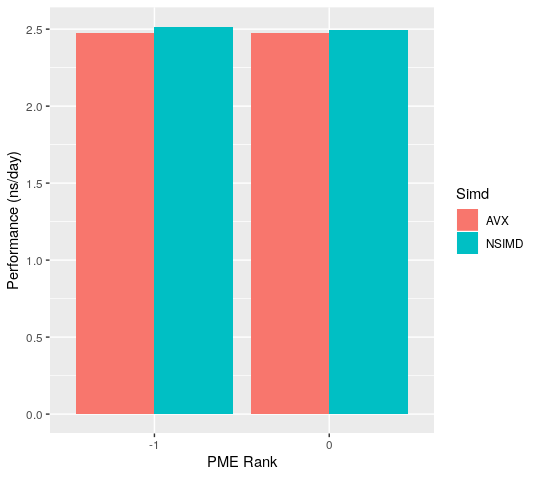
\includegraphics[scale=0.8]{AVX.png}
        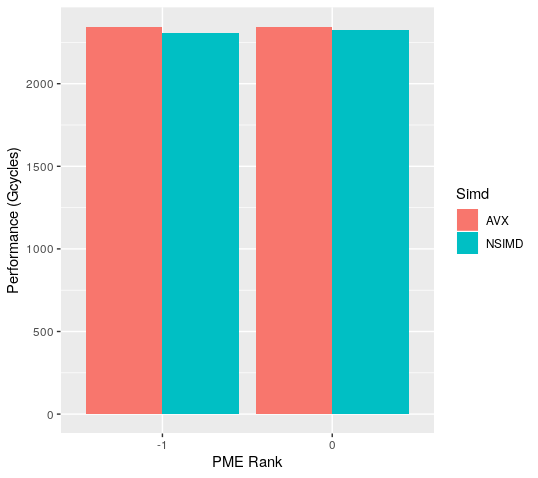
\includegraphics[scale=0.8]{AVX_2.png}
        \caption{GROMACS Performance between AVX and NSIMD}
        \label{fg:f3}
\end{figure}
\newpage

\subsection{Performance tests beetween AVX2 and NSIMD for AVX2}
\subsubsection{AVX2}
GROMACS report: \\
\begin{lstlisting}[frame=single]

------------------------------------------------------------

      P E R F O R M A N C E   R E S U L T S

------------------------------------------------------------
gmx tune_pme for GROMACS 2020-dev-20190716-2e535c390-dirty-unknown
Number of ranks         : 1
The mpirun command is   : mpirun
Passing # of ranks via  : -np
The mdrun  command is   : ./bin/gmx_mpi mdrun
mdrun args benchmarks   : -resetstep 1500 -o bench.trr -x bench.xtc -cpo bench.cpt -c bench.gro -e bench.edr -g bench.log 
Benchmark steps         : 1000
dlb equilibration steps : 1500
mdrun args at launchtime: 
Repeats for each test   : 10
Input file              : ../benches/topol.tpr
   PME/PP load estimate : 0.999978
   Number of particles  : 6
   Coulomb type         : PME
   Grid spacing x y z   : 0.115742 0.115742 0.115742
   Van der Waals type   : Cut-off

Will try these real/reciprocal workload settings:
 No.   scaling  rcoulomb  nkx  nky  nkz   spacing      rvdw  tpr file
   0  1.000000  1.000000  108  108  108  0.120000   1.000000  ../benches/topol_bench00.tpr

Individual timings for input file 0 (../benches/topol_bench00.tpr):
PME ranks      Gcycles       ns/day        PME/f    Remark
   0          2303.093        2.518          -      OK.
   0          2299.091        2.522          -      OK.
   0          2272.359        2.552          -      OK.
   0          2265.550        2.559          -      OK.
   0          2270.815        2.553          -      OK.
   0          2271.647        2.552          -      OK.
   0          2263.491        2.562          -      OK.
   0          2296.679        2.525          -      OK.
   0          2306.084        2.514          -      OK.
   0          2307.762        2.512          -      OK.
  -1( -1)     2269.441        2.555          -      OK.
  -1( -1)     2287.610        2.535          -      OK.
  -1( -1)     2269.472        2.555          -      OK.
  -1( -1)     2312.342        2.507          -      OK.
  -1( -1)     2290.687        2.531          -      OK.
  -1( -1)     2299.718        2.521          -      OK.
  -1( -1)     2272.043        2.552          -      OK.
  -1( -1)     2302.918        2.518          -      OK.
  -1( -1)     2297.881        2.523          -      OK.
  -1( -1)     2312.191        2.508          -      OK.

Tuning took    29.9 minutes.

------------------------------------------------------------
Summary of successful runs:
Line tpr PME ranks  Gcycles Av.     Std.dev.       ns/day        PME/f
   0   0    0          2285.657       18.260        2.537          -  
   1   0   -1( -1)     2291.430       16.557        2.530          -  

------------------------------------------------------------
Best performance was achieved with 0 PME ranks (see line 0)
Please use this command line to launch the simulation:

mpirun -np 1 ./bin/gmx_mpi mdrun -npme 0 -s ../benches/topol.tpr  
------------------------------------------------------------



\end{lstlisting}

Relevant information:
\begin{center}
    \begin{tabular}{|p{3.5cm}|p{3.5cm}|p{3.5cm}|p{3.5cm}|} \hline
         PME ranks & Gcycles Average & Std.dev. & ns/day \\ \hline
         0 & 2285.657  & 18.260  & 2.537  \\ \hline
         -1 (-1) & 2291.430 & 16.557 &  2.530  \\ \hline
    \end{tabular}
     \begin{tabular}{|p{3.5cm}|p{11.4cm}|} \hline
         Run Time (min) & 29.9 \\ \hline
    \end{tabular}
\end{center}

\subsubsection{NSIMD for AVX2}
GROMACS report: \\
\begin{lstlisting}[frame=single]

------------------------------------------------------------

      P E R F O R M A N C E   R E S U L T S

------------------------------------------------------------
gmx tune_pme for GROMACS 2020-dev-20190716-2e535c390-dirty-unknown
Number of ranks         : 1
The mpirun command is   : mpirun
Passing # of ranks via  : -np
The mdrun  command is   : ./gmx_mpi mdrun
mdrun args benchmarks   : -resetstep 1500 -o bench.trr -x bench.xtc -cpo bench.cpt -c bench.gro -e bench.edr -g bench.log 
Benchmark steps         : 1000
dlb equilibration steps : 1500
mdrun args at launchtime: 
Repeats for each test   : 10
Input file              : ../../benches/topol.tpr
   PME/PP load estimate : 0.999978
   Number of particles  : 6
   Coulomb type         : PME
   Grid spacing x y z   : 0.115742 0.115742 0.115742
   Van der Waals type   : Cut-off

Will try these real/reciprocal workload settings:
 No.   scaling  rcoulomb  nkx  nky  nkz   spacing      rvdw  tpr file
   0  1.000000  1.000000  108  108  108  0.120000   1.000000  ../../benches/topol_bench00.tpr

Individual timings for input file 0 (../../benches/topol_bench00.tpr):
PME ranks      Gcycles       ns/day        PME/f    Remark
   0          2239.504        2.589          -      OK.
   0          2217.979        2.614          -      OK.
   0          2221.664        2.610          -      OK.
   0          2220.557        2.611          -      OK.
   0          2216.868        2.615          -      OK.
   0          2235.613        2.594          -      OK.
   0          2217.337        2.615          -      OK.
   0          2237.331        2.592          -      OK.
   0          2215.275        2.617          -      OK.
   0          2222.848        2.608          -      OK.
  -1( -1)     2213.238        2.620          -      OK.
  -1( -1)     2213.839        2.619          -      OK.
  -1( -1)     2944.781        1.969          -      OK.
  -1( -1)     2252.241        2.574          -      OK.
  -1( -1)     2246.926        2.580          -      OK.
  -1( -1)     2216.212        2.616          -      OK.
  -1( -1)     2563.122        2.262          -      OK.
  -1( -1)     2239.827        2.589          -      OK.
  -1( -1)     2258.836        2.567          -      OK.
  -1( -1)     2242.114        2.586          -      OK.

Tuning took    29.4 minutes.

------------------------------------------------------------
Summary of successful runs:
Line tpr PME ranks  Gcycles Av.     Std.dev.       ns/day        PME/f
   0   0    0          2224.498        9.290        2.607          -  
   1   0   -1( -1)     2339.114      236.975        2.498          -  

------------------------------------------------------------
Best performance was achieved with 0 PME ranks (see line 0)
Please use this command line to launch the simulation:

mpirun -np 1 ./gmx_mpi mdrun -npme 0 -s ../../benches/topol.tpr  
------------------------------------------------------------


\end{lstlisting}

Relevant information:
\begin{center}
    \begin{tabular}{|p{3.5cm}|p{3.5cm}|p{3.5cm}|p{3.5cm}|} \hline
         PME ranks & Gcycles Average & Std.dev. & ns/day \\ \hline
         0 & 2224.498  & 9.290  & 2.607  \\ \hline
         -1 (-1) & 2339.114 & 236.975 & 2.498  \\ \hline
    \end{tabular}
     \begin{tabular}{|p{3.5cm}|p{11.4cm}|} \hline
         Run Time (min) & 29.4 \\ \hline
    \end{tabular}
\end{center}
\subsubsection{Comparison of results}

\begin{figure}[!h]
\centering
        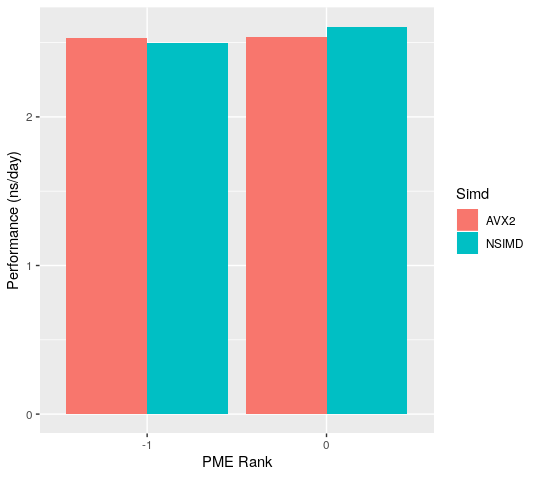
\includegraphics[scale=0.8]{AVX2.png}
        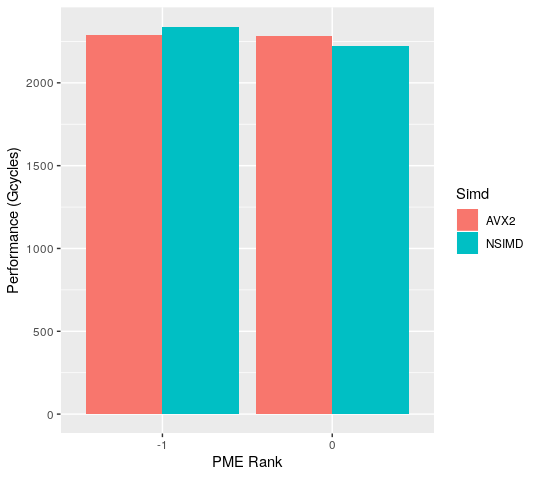
\includegraphics[scale=0.8]{AVX2_2.png}
        \caption{GROMACS Performance between AVX2 and NSIMD}
        \label{fg:f4}
\end{figure}
\newpage

\subsection{Performance tests between AVX512 Skylake and NSIMD}
\subsubsection{AVX512 Skylake}
GROMACS report: \\
\begin{lstlisting}[frame=single]

------------------------------------------------------------

      P E R F O R M A N C E   R E S U L T S

------------------------------------------------------------
gmx tune_pme for GROMACS 2020-dev-20190716-2e535c390-dirty-unknown
Number of ranks         : 1
The mpirun command is   : mpirun
Passing # of ranks via  : -np
The mdrun  command is   : ../build/bin/gmx_mpi mdrun
mdrun args benchmarks   : -resetstep 1500 -o bench.trr -x bench.xtc -cpo bench.cpt -c bench.gro -e bench.edr -g bench.log 
Benchmark steps         : 1000
dlb equilibration steps : 1500
mdrun args at launchtime: 
Repeats for each test   : 10
Input file              : topol.tpr
   PME/PP load estimate : 0.999978
   Number of particles  : 6
   Coulomb type         : PME
   Grid spacing x y z   : 0.115742 0.115742 0.115742
   Van der Waals type   : Cut-off

Will try these real/reciprocal workload settings:
 No.   scaling  rcoulomb  nkx  nky  nkz   spacing      rvdw  tpr file
   0  1.000000  1.000000  108  108  108  0.120000   1.000000  topol_bench00.tpr

Individual timings for input file 0 (topol_bench00.tpr):
PME ranks      Gcycles       ns/day        PME/f    Remark
   0          2897.292        2.001          -      OK.
   0          2844.918        2.038          -      OK.
   0          2847.273        2.036          -      OK.
   0          2843.928        2.039          -      OK.
   0          2837.601        2.043          -      OK.
   0          2845.022        2.038          -      OK.
   0          2828.695        2.050          -      OK.
   0          2840.640        2.041          -      OK.
   0          2875.328        2.017          -      OK.
   0          2900.729        1.999          -      OK.
  -1( -1)     2870.352        2.020          -      OK.
  -1( -1)     2910.020        1.992          -      OK.
  -1( -1)     2840.259        2.041          -      OK.
  -1( -1)     2837.620        2.043          -      OK.
  -1( -1)     2836.012        2.044          -      OK.
  -1( -1)     2848.980        2.035          -      OK.
  -1( -1)     2878.510        2.014          -      OK.
  -1( -1)     2849.192        2.035          -      OK.
  -1( -1)     2848.824        2.035          -      OK.
  -1( -1)     2834.264        2.046          -      OK.

Tuning took    36.6 minutes.

------------------------------------------------------------
Summary of successful runs:
Line tpr PME ranks  Gcycles Av.     Std.dev.       ns/day        PME/f
   0   0    0          2856.143       25.526        2.030          -  
   1   0   -1( -1)     2855.403       24.111        2.030          -  

------------------------------------------------------------
Best performance was achieved with the automatic number of PME ranks (see line 1)
Please use this command line to launch the simulation:

mpirun -np 1 ../build/bin/gmx_mpi mdrun -npme -1 -s topol.tpr  
------------------------------------------------------------

\end{lstlisting}


Relevant information:
\begin{center}
    \begin{tabular}{|p{3.5cm}|p{3.5cm}|p{3.5cm}|p{3.5cm}|} \hline
         PME ranks & Gcycles Average & Std.dev. & ns/day \\ \hline
         0 & 2856.143  & 25.526  & 2.030  \\ \hline
         -1 (-1) & 2855.403 & 24.111 & 2.030  \\ \hline
    \end{tabular}
     \begin{tabular}{|p{3.5cm}|p{11.4cm}|} \hline
         Run Time (min) & 36.6 \\ \hline
    \end{tabular}
\end{center}
\subsubsection{NSIMD for AVX512 Skylake}
GROMACS report: \\
\begin{lstlisting}[frame=single]

------------------------------------------------------------

      P E R F O R M A N C E   R E S U L T S

------------------------------------------------------------
gmx tune_pme for GROMACS 2020-dev-20190716-2e535c390-dirty-unknown
Number of ranks         : 1
The mpirun command is   : mpirun
Passing # of ranks via  : -np
The mdrun  command is   : ../build/bin/gmx_mpi mdrun
mdrun args benchmarks   : -resetstep 1500 -o bench.trr -x bench.xtc -cpo bench.cpt -c bench.gro -e bench.edr -g bench.log 
Benchmark steps         : 1000
dlb equilibration steps : 1500
mdrun args at launchtime: 
Repeats for each test   : 10
Input file              : topol.tpr
   PME/PP load estimate : 0.999978
   Number of particles  : 6
   Coulomb type         : PME
   Grid spacing x y z   : 0.115742 0.115742 0.115742
   Van der Waals type   : Cut-off

Will try these real/reciprocal workload settings:
 No.   scaling  rcoulomb  nkx  nky  nkz   spacing      rvdw  tpr file
   0  1.000000  1.000000  108  108  108  0.120000   1.000000  topol_bench00.tpr

Individual timings for input file 0 (topol_bench00.tpr):
PME ranks      Gcycles       ns/day        PME/f    Remark
   0          2891.051        2.006          -      OK.
   0          2864.722        2.024          -      OK.
   0          2847.975        2.036          -      OK.
   0          2835.103        2.045          -      OK.
   0          2823.214        2.054          -      OK.
   0          2842.263        2.040          -      OK.
   0          2835.411        2.045          -      OK.
   0          2856.506        2.030          -      OK.
   0          2892.082        2.005          -      OK.
   0          2892.229        2.005          -      OK.
  -1( -1)     2853.384        2.032          -      OK.
  -1( -1)     2855.301        2.031          -      OK.
  -1( -1)     2829.456        2.049          -      OK.
  -1( -1)     2828.396        2.050          -      OK.
  -1( -1)     2870.420        2.020          -      OK.
  -1( -1)     2822.364        2.054          -      OK.
  -1( -1)     2896.988        2.001          -      OK.
  -1( -1)     2891.035        2.006          -      OK.
  -1( -1)     2909.175        1.993          -      OK.
  -1( -1)     2801.228        2.070          -      OK.

Tuning took    36.5 minutes.

------------------------------------------------------------
Summary of successful runs:
Line tpr PME ranks  Gcycles Av.     Std.dev.       ns/day        PME/f
   0   0    0          2858.056       25.961        2.029          -  
   1   0   -1( -1)     2855.775       35.820        2.031          -  

------------------------------------------------------------
Best performance was achieved with the automatic number of PME ranks (see line 1)
Please use this command line to launch the simulation:

mpirun -np 1 ../build/bin/gmx_mpi mdrun -npme -1 -s topol.tpr  
------------------------------------------------------------

\end{lstlisting}


Relevant information:
\begin{center}
    \begin{tabular}{|p{3.5cm}|p{3.5cm}|p{3.5cm}|p{3.5cm}|} \hline
         PME ranks & Gcycles Average & Std.dev. & ns/day \\ \hline
         0 & 2858.056  & 25.961  & 2.029  \\ \hline
         -1 (-1) & 2855.775 & 35.820 & 2.031 \\ \hline
    \end{tabular}
     \begin{tabular}{|p{3.5cm}|p{11.4cm}|} \hline
         Run Time (min) & 36.5 \\ \hline
    \end{tabular}
\end{center}

\subsubsection{Comparison of results}

\begin{figure}[!h]
\centering
        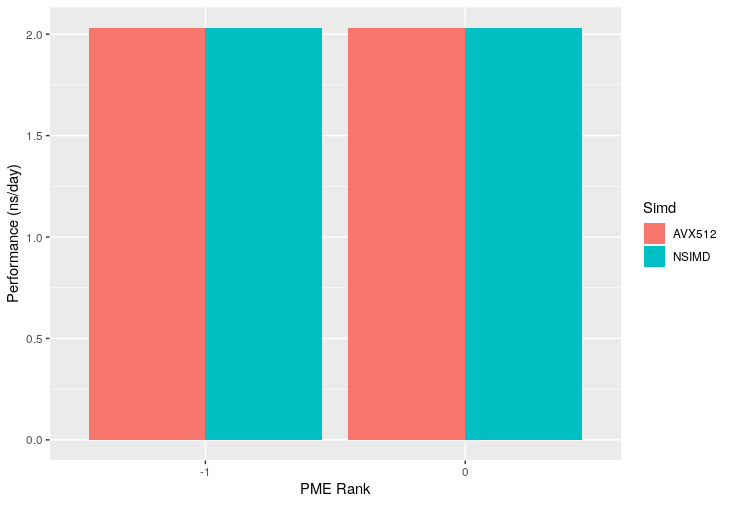
\includegraphics[scale=0.8]{AVX512.png}
        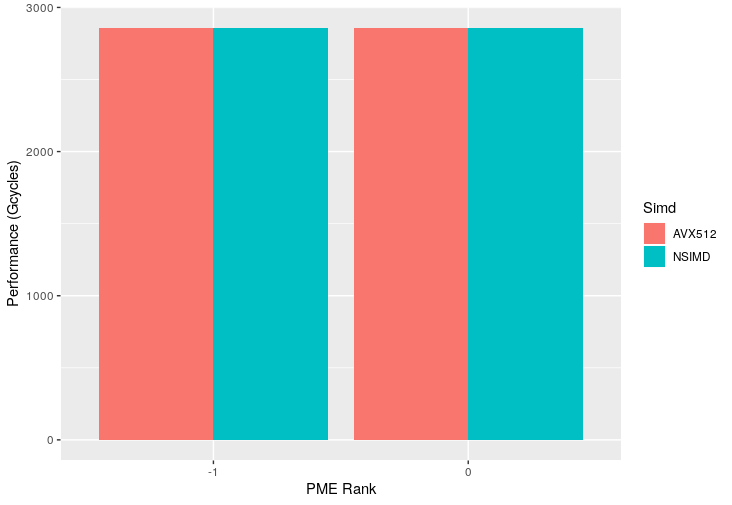
\includegraphics[scale=0.8]{AVX512_2.png}
        \caption{GROMACS Performance between AVX 512 and NSIMD}
        \label{fg:f5}
\end{figure}

\bibliography{references}
\bibliographystyle{unsrt}
\end{document}


